\chapter{Design and Methodology}
\label{chap:design_methodology}

This chapter includes a comprehensive review of the design and methods used adopted for developing the AI-driven medical chatbot. The system is tailored to cater to two distinct cohorts: patients and students of medicine, approached from an educational standpoint and pragmatic support including symptom evaluation and independent management of appointments. The complete system flow and design are shown in Figure 3.1.

\section{High-Level Architecture}
\label{sec:high_level_architecture}

The system is structured into several interconnected modules, as shown in Figure 3.1.
\begin{figure}[htbp]
    \begin{center}
      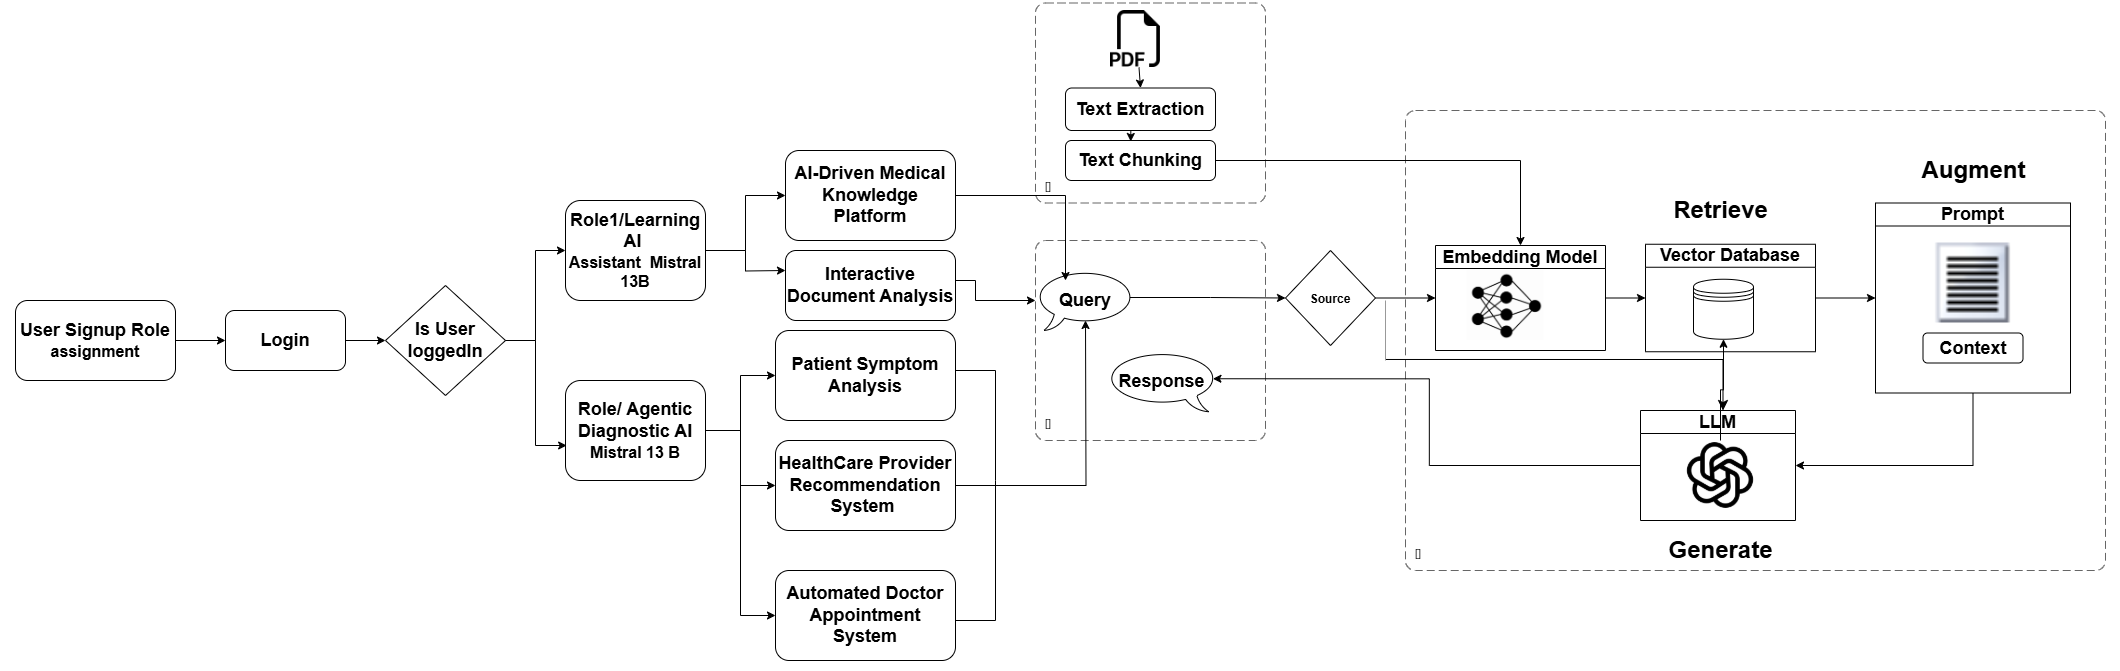
\includegraphics[width=16cm,height=10cm]{./Images/Thesis.png}
       \caption{Thesis implementation phases}
       \label{fig: Thesis implementation phases}
    \end{center}
\end{figure}

\vspace{2cm}
\begin{enumerate}
  \item \textbf{User Authentication and Role Identification:} 
    \begin{itemize}
        \item Upon user login, the system authenticates and decides the individual's role as either medical student or patient.
        \item Role-based access controls the assignment of users to a particular dashboard and capabilities.
    \end{itemize}
  \item \textbf{Role-Based Interaction:} 
    \begin{itemize}
        \item \emph{Medical Student Mode:} Medical Student Mode: Provides exhaustive study aids such as PDF files with scholarly question-and-answer sessions.
        \item \emph{Patient Mode:} Gives a symptom analysis with suggestions for location based doctor recommendation with agentic appointment system.
    \end{itemize}
  \item \textbf{PDF Processing and Text Chunking:} 
    \begin{itemize}
        \item Extracts text from uploaded PDFs and segments them into manageable chunks for embedding and retrieval.
    \end{itemize}
  \item \textbf{Embedding and Vector Storage:}
    \begin{itemize}
        \item Uses \texttt{all-mpnet-base-v2} for semantic embeddings.
        \item Stores embeddings in a vector database (\emph{Pinecone}) for efficient similarity-based retrieval.
    \end{itemize}
  \item \textbf{Retrieval-Augmented Generation (RAG):} 
    \begin{itemize}
        \item User queries are embedded and matched against stored vectors to retrieve relevant chunks.
        \item The retrieved context is then used to generate accurate responses using the \textbf{Mistral 13B Quantized Model}.
    \end{itemize}
  \item \textbf{LLM Response Generation:}
    \begin{itemize}
        \item The Mistral 13B Quantized Model generates context-aware, role-specific answers.
        \item Responses are tailored differently for educational depth (students) and practical advice (patients).
    \end{itemize}
  \item \textbf{Agentic Appointment Booking:}
    \begin{itemize}
        \item For patients, the system autonomously schedules appointments by integrating healthcare provider data.
    \end{itemize}
\end{enumerate}

\section{Mistral 13B Quantized Model}
\label{sec:mistral_model}

The \textbf{Mistral 13B Quantized Model} serves as the core LLM for generating responses. It is chosen for its balance between performance and computational efficiency.

\subsection{Overview and Architecture}
\label{subsec:mistral_overview}
The Mistral 13B Quantized Model is a variant of the Mistral architecture known for:
\begin{itemize}
    \item \textbf{Parameter Efficiency:} With 13 billion parameters, it achieves high performance while maintaining manageable resource requirements due to quantization.
    \item \textbf{Quantization Technique:} Utilizes Q3\_K\_M quantization, reducing memory footprint and speeding up inference without significantly sacrificing accuracy.
    \item \textbf{Transformer Architecture:} Built on a decoder-only architecture with multi-head self-attention and feed-forward layers, optimized for generative tasks.
\end{itemize}

\subsection{Contextual Response Generation}
\label{subsec:mistral_response}
\begin{itemize}
    \item The model generates responses by leveraging the context retrieved through the \emph{RAG} pipeline.
    \item Role-specific prompts guide the model in generating:
        \begin{itemize}
            \item \emph{Educational Explanations} for medical students with detailed references.
            \item \emph{Simple, Actionable Advice} for patients, ensuring clarity and minimizing jargon.
        \end{itemize}
\end{itemize}

\subsection{Role-Specific Prompting}
\label{subsec:mistral_prompting}
Different prompts are crafted based on user roles:
\begin{itemize}
    \item \textbf{For Medical Students:}
        \begin{itemize}
            \item Requests comprehensive explanations with references to academic sources.
            \item Example: “Explain the mechanism of action of beta-blockers with clinical implications.”
        \end{itemize}
    \item \textbf{For Patients:}
        \begin{itemize}
            \item Prompts the model to generate concise, easy-to-understand guidance.
            \item Example: “What should I do if I experience chest pain?”
        \end{itemize}
\end{itemize}

\subsection{Additional Explanation of the Mistral 13B Quantized Model}
\label{subsec:mistral_explanation}
The Mistral 13B Quantized Model has been specifically chosen for this system due to its excellent balance between computational efficiency and high-quality response generation. The quantization process significantly reduces the model’s memory footprint and speeds up inference times, which is critical for delivering real-time responses in a production environment. Despite its compact size, the model maintains robust performance across diverse tasks, making it well-suited for both the detailed educational requirements of medical students and the clear, actionable advice needed by patients.

\section{Embedding and Vector Database}
\label{sec:embedding_vector_db}

\subsection{Embedding Model: \texttt{all-mpnet-base-v2}}
\label{subsec:all_mpnet_base_v2}
\texttt{all-mpnet-base-v2} is employed for converting text chunks and queries into 768-dimensional embeddings. Key features include:
\begin{itemize}
  \item \textbf{Contextual Semantic Representation:} Captures contextual meaning, enhancing query relevance.
  \item \textbf{Performance:} Consistently outperforms older models (like BERT) in semantic search tasks.
  \item \textbf{Compatibility:} Embeddings are stored in \emph{Pinecone} for rapid cosine similarity-based searches.
\end{itemize}

\subsection{Vector Database: Pinecone}
\label{subsec:pinecone}
\emph{Pinecone} is chosen as the vector database for its robust performance in managing high-dimensional embeddings and its seamless integration within the retrieval pipeline. Key features include:
\begin{itemize}
    \item \textbf{Scalability:} Pinecone is designed to efficiently index and manage millions of embeddings, ensuring low-latency retrieval even as the data volume grows. This scalability makes it ideal for applications with rapidly expanding datasets.
    \item \textbf{Metric Support:} By utilizing cosine similarity as the primary metric for relevance ranking, Pinecone delivers highly accurate and meaningful search results, which are critical for ensuring that the most contextually relevant information is retrieved.
    \item \textbf{High Performance:} The database is optimized for speed, enabling real-time searches and updates. This is essential for applications requiring immediate responses, such as the medical chatbot system.
    \item \textbf{Integration with Retrieval Pipelines:} Pinecone seamlessly integrates with frameworks like LangChain, simplifying the process of embedding storage and retrieval. This tight integration helps maintain a smooth workflow from query embedding to final response generation.
    \item \textbf{Reliability and Consistency:} Pinecone offers a reliable infrastructure that ensures data consistency and durability, which is critical for systems handling sensitive and large-scale information.
    \item \textbf{Ease of Use:} With a user-friendly API and robust documentation, Pinecone enables developers to implement and manage the vector database with minimal overhead, facilitating faster development cycles.
\end{itemize}


\section{Agentic Appointment Booking}
\label{sec:agentic_booking}

\subsection{Triggering Conditions and Workflow}
\label{subsec:booking_workflow}
The system autonomously handles appointment booking by:
\begin{enumerate}
    \item Detecting user intent through keywords (e.g., “book an appointment”).
    \item Collecting details like location and specialty.
    \item Querying a dynamic dataset of 7,000+ healthcare providers scraped from Bing Maps.
    \item Generating a booking link via Doctolib and sending it through Twilio SMS integration.
\end{enumerate}

\section{User Interface Approaches}
\label{sec:user_interface}

\subsection{Flask UI}
\label{subsec:flask_ui}
\emph{Flask} is used for:
\begin{itemize}
    \item \textbf{User Authentication:} Role-based access control for students and patients.
    \item \textbf{File Upload:} Allowing PDF uploads for medical students.
    \item \textbf{Query Form:} Basic input form for submitting questions.
\end{itemize}

The Flask UI is designed to handle user authentication, registration, and file uploads seamlessly. It also integrates with a separate Chainlit process that provides a chat-centric interface. Upon successful login, Flask starts Chainlit in a new thread, passing the user's email via environment variables so that Chainlit can fetch role-specific details from the database. This integration ensures that users are quickly redirected to a dynamic and responsive chatbot interface after authentication.

\subsection{Chainlit UI}
\label{subsec:chainlit_ui}
\emph{Chainlit} provides a chat-centric interface designed to enhance user engagement through interactive and dynamic conversation flows. Key features include:
\begin{itemize}
    \item \textbf{Role-Specific Chat Profiles:} The system supports different conversation modes tailored for medical students and patients. Each profile presents customized prompts and responses, ensuring that the dialogue remains relevant to the user's context—whether that involves detailed academic discussions or clear, actionable health advice.
    \item \textbf{Interactive Conversation Elements:} Chainlit UI incorporates features such as real-time feedback, adaptive conversation threads, and dynamic content loading. This enables users to interact fluidly with the chatbot, with the interface automatically adjusting based on user input and query context.
    \item \textbf{Enhanced User Engagement:} By integrating multimedia elements and interactive buttons, Chainlit helps to create a more engaging experience. For example, users can click on suggested topics or follow-up questions, which makes navigating complex information more intuitive.
    \item \textbf{Seamless Integration with Back-End Systems:} The UI is designed to work in tandem with the underlying retrieval and generation pipelines. It receives context-aware responses from the \textbf{Mistral 13B Quantized Model} and displays them in an easily digestible format, while also allowing users to refine or extend their queries interactively.
    \item \textbf{Customization and Scalability:} The modular design of Chainlit allows for easy customization of chat elements and conversation flows. This flexibility supports ongoing improvements and scalability as new features are integrated or as user needs evolve.
\end{itemize}


\section{Summary}
\label{sec:methodology_summary}
In summary, this chapter outlines a robust design for an AI-driven medical chatbot that effectively serves two distinct user groups: medical students and patients. The system's modular architecture incorporates user authentication, PDF processing, semantic embedding using \texttt{all-mpnet-base-v2}, and a vector database via Pinecone for rapid retrieval. A retrieval-augmented generation pipeline seamlessly integrates the powerful \textbf{Mistral 13B Quantized Model} to generate context-aware responses. Furthermore, the solution provides specialized functionalities, such as role-based interaction and autonomous appointment booking, ensuring that educational and practical needs are both addressed efficiently. The integration between the Flask UI and the Chainlit chat interface is a key component, enabling dynamic, real-time engagement that leverages user-specific data to tailor responses and services. The next chapter will delve into the implementation details, system deployment, and further integration strategies.

